\documentclass{article}
\usepackage[english]{babel}
\usepackage[utf8]{inputenc}
\usepackage{fancyhdr}
\usepackage[top=1.25in, bottom=1.25in, right=1in, left=1in]{geometry}
\usepackage{graphicx}
\usepackage{filecontents}
\usepackage{amsmath,amsfonts,amssymb,amsthm}
\usepackage{mathtools}
\usepackage{commath}
\usepackage{gauss}
\usepackage{enumerate}

\usepackage{etoolbox}
\makeatletter
\patchcmd\g@matrix
 {\vbox\bgroup}
 {\vbox\bgroup\normalbaselines}% restore the standard baselineskip
 {}{}
\makeatother

\pagestyle{fancy}
\fancyhf{}
\rhead{Introduction to Data Science}
\lhead{Predicting Electricity Spot Price}
\rfoot{Page \thepage}
\makeatletter
\renewcommand{\@seccntformat}[1]{}
\makeatother 

%% Theorems etc. %%%%%%%%%%%%%%
%\swapnumbers
\numberwithin{equation}{section}

\makeatletter
\let\c@equation\c@subsection
\makeatother

\title{%
	Predicting Electricity Spot Price\\
	\large Introduction to Data Science Course Project}
\author{Ville Pirsto, Emil Tigerstedt, Ahsan Abbas}

\begin{document}

% Titlepage separately
\begin{titlepage}
	\maketitle
	\thispagestyle{empty}
\end{titlepage}

\tableofcontents
\clearpage

% ---- Introduction ----
\section{Introduction}
This is the introduction that should contain some pretty general stuff. Below, some initial suggestions are listed.
\begin{itemize}
	\item What was done?
	\item Why? Motivation (canvas)
	\item How? 
	\item Summary of the results
\end{itemize}

% ---- Canvas ----
\section{Project Work Canvas}
\textbf{Note: this is just the canvas template, to be replaced with our filled canvas.}
\begin{figure}[htb]
	\centering
	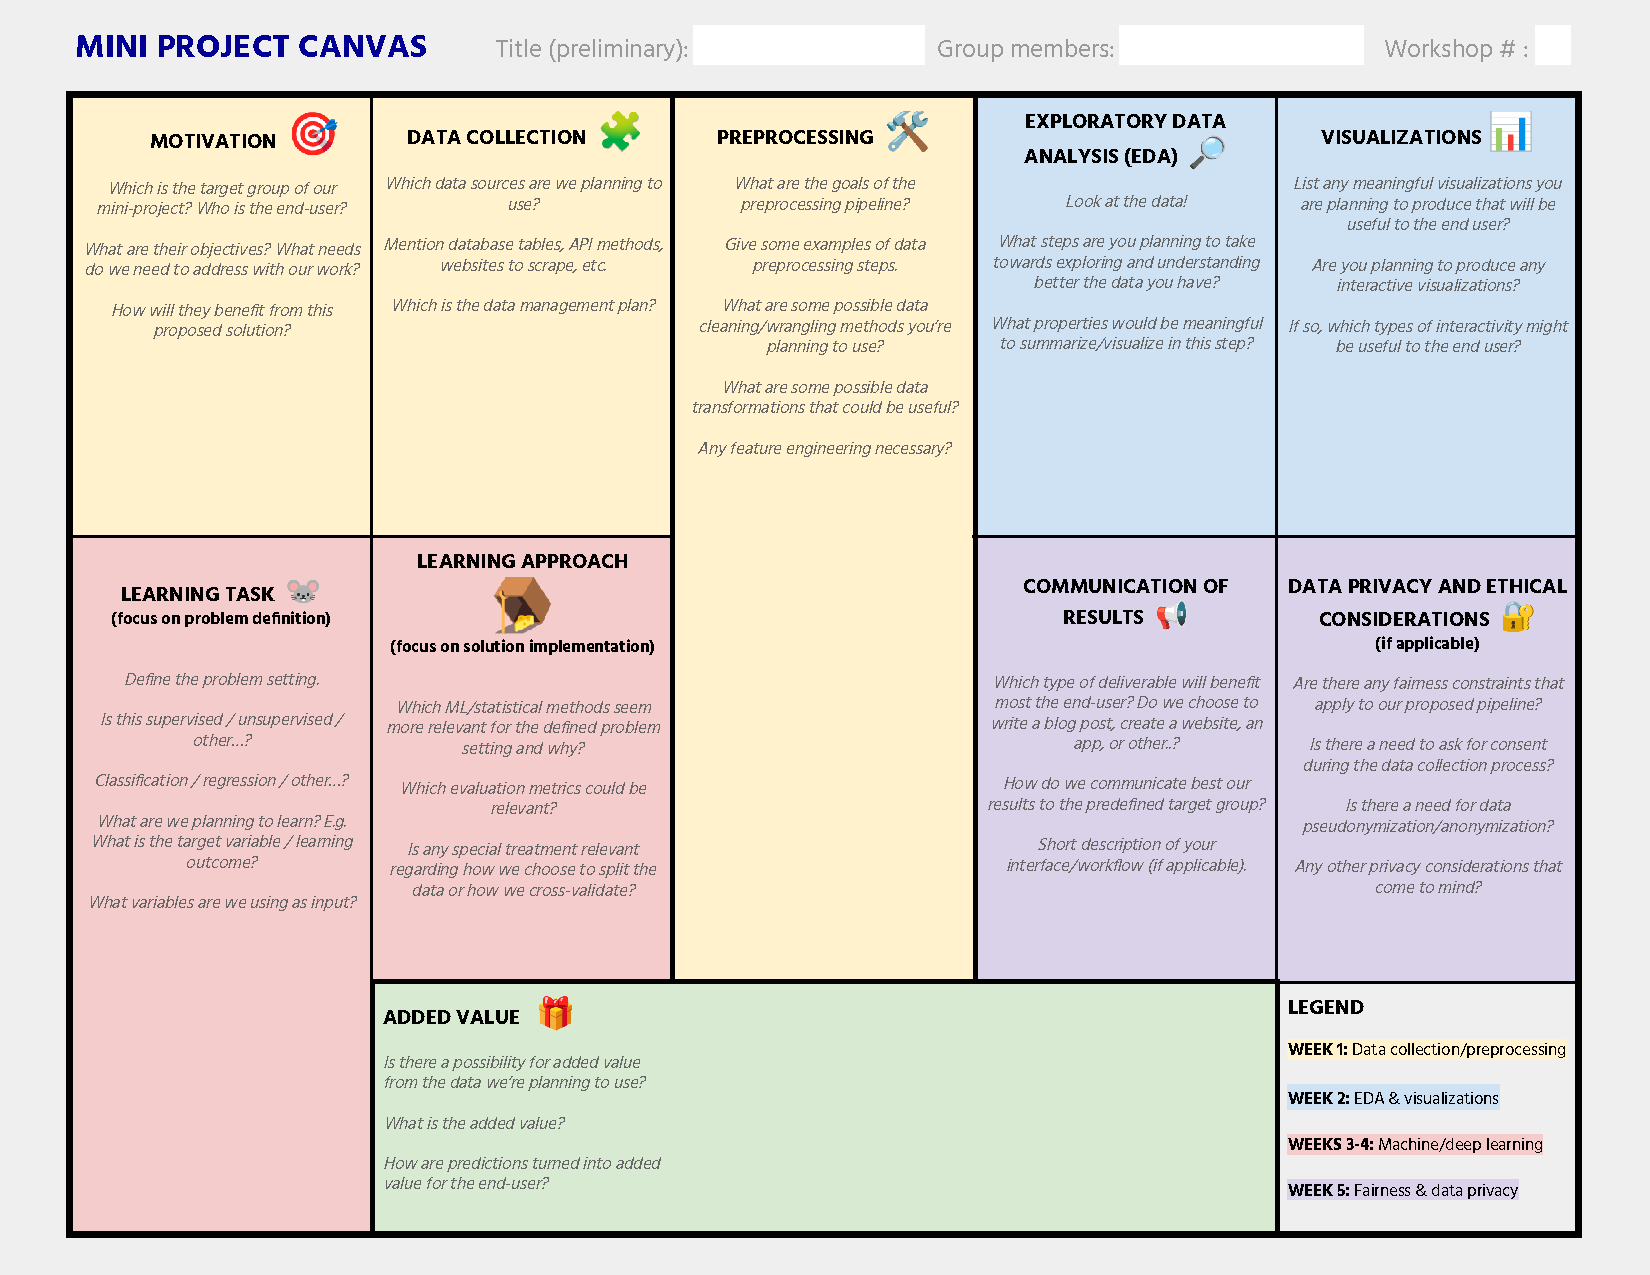
\includegraphics[width=1\textwidth]{./mini_project_canvas.pdf}
	\caption{Canvas used for project planning.}
	\label{fig1}
\end{figure}

% ---- Data Collection and Preprocessing ----
\section{Data Collection and Preprocessing}
\begin{itemize}
	\item Where is data used from?
	\item How is data stored?
	\item What kind of data is used?
	\item How is data accessed?
	\item What kind of preprocessing is done?
\end{itemize}

% ---- EDA and Visualizations ----
\section{Exploratory Data Analysis and Visualizations}
\begin{itemize}
	\item What kind of EDA was done?
	\item How was the data visualized?
	\item What kind of findings were obtained?
\end{itemize}

% ---- Learning ----
\section{Learning to Predict Electricity Spot prices}
\begin{itemize}
	\item What kind of approaches were tried?
	\item What kind of observations were made during this process?
	\item What approach was used in the end? Why? How did we end up to it?
\end{itemize}

% ---- Communciation of Results ----
\section{Communication of Results}
\begin{itemize}
	\item Webpage, how?
	\item What kind of user interface is used?
	\item What does the webpage do? What can the user do?
\end{itemize}

% ---- Summary ----
\section{Summary}
\begin{itemize}
	\item Predicting electricity spot prices is difficult
	\item Nevertheless, a decent method was found for the used input variables
	\item We learned alot, maybe list here someof the thigs that we discussed
	\item What could be done better / future continuation topics
\end{itemize}


% ----------------------------------------------------------------
\iffalse
\begin{figure}[htb]
\centering
\includegraphics[width=.5\textwidth]{./largestEigenvalue.eps}
\caption{Suurimman ominaisarvon approksimaatiovirheen itseisarvo $i$:n funktiona.}
\label{fig1}
\end{figure}
\fi

\end{document}